
\documentclass[a4paper]{article}

%\hypersetup{colorlinks} % Comment this line if you don't wish to have colored links

\usepackage{microtype} % Improves character and word spacing

%\usepackage{lipsum} % Inserts dummy text

\usepackage{booktabs} % Better horizontal rules in tables
\usepackage[spanish]{babel}

\usepackage{float}

\usepackage[utf8]{inputenc}

\usepackage{amsmath}
\usepackage{geometry}

\usepackage{graphicx} % Needed to insert images into the document
\graphicspath{{graphics/}} % Sets the default location of pictures
\setkeys{Gin}{width=\linewidth,totalheight=\textheight,keepaspectratio} % Improves figure scaling

\usepackage{fancyvrb} % Allows customization of verbatim environments

\geometry{
	a4paper,
	total={170mm,257mm},
	left=30mm,
	top=20mm,
	textwidth=158mm,
}

\usepackage{xspace} % Used for printing a trailing space better than using a tilde (~) using the \xspace command

\newcommand{\monthyear}{\ifcase\month\or January\or February\or March\or April\or May\or June\or July\or August\or September\or October\or November\or December\fi\space\number\year} % A command to print the current month and year


\newcommand{\blankpage}{\newpage\hbox{}\thispagestyle{empty}\newpage} % Command to insert a blank page
\renewcommand*\contentsname{Contenidos}
\renewcommand*\listfigurename{Lista de Figuras}
\renewcommand*\listtablename{Lista de tablas}
\renewcommand*\figurename{Figura}
\renewcommand*\tablename{Tabla}
\renewcommand{\partname}{Parte}

%\newenvironment{myfont}{\fontfamily{<Windows Lucida Console>}\selectfont}{\par}
%\DeclareTextFontCommand{\textmyfont}{\myfont}

%\usepackage{units} % Used for printing standard units

\usepackage{color}
\definecolor{javared}{rgb}{0.6,0,0} % for strings
\definecolor{javagreen}{rgb}{0.25,0.5,0.35} % comments
\definecolor{javapurple}{rgb}{0.5,0,0.35} % keywords
\definecolor{javadocblue}{rgb}{0.25,0.35,0.75} % javadoc

\newcommand{\HRule}[1]{\rule{\linewidth}{#1}}
\renewcommand*\ttdefault{cmvtt}
%\usepackage{ascii}

\usepackage{fontenc}

\usepackage{listings}
\lstset{
	language=Java,
	basicstyle=\small,
	keywordstyle=\color{javapurple}\bfseries,
	stringstyle=\color{javared},
	commentstyle=\color{javagreen},
	morecomment=[s][\color{javadocblue}]{/**}{*/},
	numbers=left,
	numberstyle=\tiny\color{black},
	stepnumber=1,
	numbersep=8pt,
	tabsize=2,
	showspaces=false,
	showstringspaces=false
}


\usepackage{makeidx} % Used to generate the index
\makeindex % Generate the index which is printed at the end of the document

%----------------------------------------------------------------------------------------
%	BOOK META-INFORMATION
%----------------------------------------------------------------------------------------

\title{Evaluación de prestaciones de algoritmos conscientes de la red para la planificación de contenedores ligeros sobre infraestructuras paralelas distribuidas } % Title of the book

\author{Ángel Roberto García Serpa} % Author

%----------------------------------------------------------------------------------------

\begin{document}
		\begin{titlepage}
		\centering
		
		\vspace{3.5cm}
		
		
\includegraphics[width=0.2\textwidth]{graphics/logo_uned}
		
		\vspace{3.5cm}
		
		
		\HRule{3pt} \\ [0.5cm]
		
		{\huge\bfseries Evaluación de prestaciones de algoritmos conscientes de la red para la planificación de contenedores ligeros sobre infraestructuras paralelas distribuidas\par}
		\vspace{4cm}
		{\Large\itshape Ángel Roberto García Serpa\par}
		\vspace{4cm}
		\begin{flushleft}
			
		
		\textbf{Asignatura:} 71013035 – Diseño de Software\\
		\textbf{Año de la práctica:} 2019-2020\\
		\textbf{Centro Asociado al que pertenece:} 160016 - Bogotá,\\
		\textbf{Tutor que le da asistencia:}\\ 
		\textbf{Datos personales:}\\ 
		\textbf{Nombre y apellidos:} Ángel Roberto García Serpa\\
		\textbf{DNI:} 52539216V\\
		\textbf{Contacto:} 683596728 - argserpa@gmail.com\\
		\textbf{Localidad de residencia:} Ciempozuelos, Madrid\\
		\textbf{Datos de coste:}\\
  		\textbf{Horas de dedicación al estudio de los contenidos}:  30\\
		\textbf{Nº de actividades no evaluables realizadas y horas de dedicación:} 0.0\\
		\textbf{Horas de dedicación para realizar esta actividad:}  20\\
	\end{flushleft}		
		\vfill		
		% Bottom of the page
		{\large 25 de agosto de 2020\par}
	\end{titlepage}


	
	\newpage

	
	
	%----------------------------------------------------------------------------------------
	
	\tableofcontents % Print the table of contents
	
	%----------------------------------------------------------------------------------------
	
	\listoffigures % Print a list of figures	
	\pagebreak
	
\part{Enunciado y planteamiento del caso de estudio.}
\paragraph{}El escenario en el que se situará el funcionamiento del caso de uso (pregunta 2), consiste en un paquete para la \textbf{gestión \underline{sanitaria} de una explotación ganadera.} (SanGranja).
\paragraph{}Dicho módulo (o paquete) forma parte de una aplicación dedicada a la gestión \underline{integral} ganadera (i-FarM).
\paragraph{}El negocio general del usuario de estas aplicaciones es el cuidado y la cría de animales para el consumo humano de sus productos.
\paragraph{}Esta descripción del escenario, en el que se ubica el caso de uso que se va a implementar en el ejercicio, se refiere al módulo {\large SanGranja}. Lógicamente, interactúa con algunos de los servicios que provee {\large i-FarM} (considerado externo a {\large SanGranja}) pero, también, con otros servicios aportados por sistemas de apoyo externos (como el Sistema de Gestión del Almacén común con toda la Información –Datos– del sistema integral que, además, también daría soporte a {\large i-FarM}).



\paragraph{}De esta forma, el propósito fundamental del módulo {\large SanGranja} es ocuparse de:
\begin{itemize}
	\item La gestión {\large Sanitaria}  de los animales y de las instalaciones. Es decir, de la monitorización, diagnóstico, {\large tratamiento} y seguimiento de la salud de cada animal.
\end{itemize}
\paragraph{}El ciclo vital de cada individuo suele transcurrir en unas instalaciones o recintos ({\large corrales}) en los que se supervisan sus condiciones ambientales, la alimentación especializada o los tratamientos sanitarios que recibe. Para realizar esta funcionalidad, se va a suponer que cada animal lleva implantado un dispositivo biométrico que recoge la información necesaria. Estos datos se mantienen en el {\large Sistema de Información} global de la explotación, en la parte que le corresponde tanto a {\large i-FarM} como a {\large SanGranja},.

\paragraph{}De la misma manera que ocurre con la aplicación general {\large i-FarM},\textbf{ el objetivo fundamental de la construcción del módulo SanGranja es que}, además de funcionar colaborativa e independientemente de {\large i-FarM}, \textbf{sea fácilmente escalable y adaptable a la dimensión de la explotación, a la estructura organizativa con que se realiza, a la naturaleza de su ganadería, a las enfermedades que les afectan y a sus tratamientos}.
\paragraph{}




\newpage
\part{Resolución del problema.}
\section{Sección 1.\\Evaluación de los Casos de Uso}
\subsection{Ej 1. (0’5 puntos)}
Represente, en un diagrama UML de casos de uso, los casos de uso primarios (Elementary Business Process) más importantes, sus actores principales, los de apoyo y las interacciones correspondientes para el módulo SanGranja.
\begin{figure}[H]
	\centering
	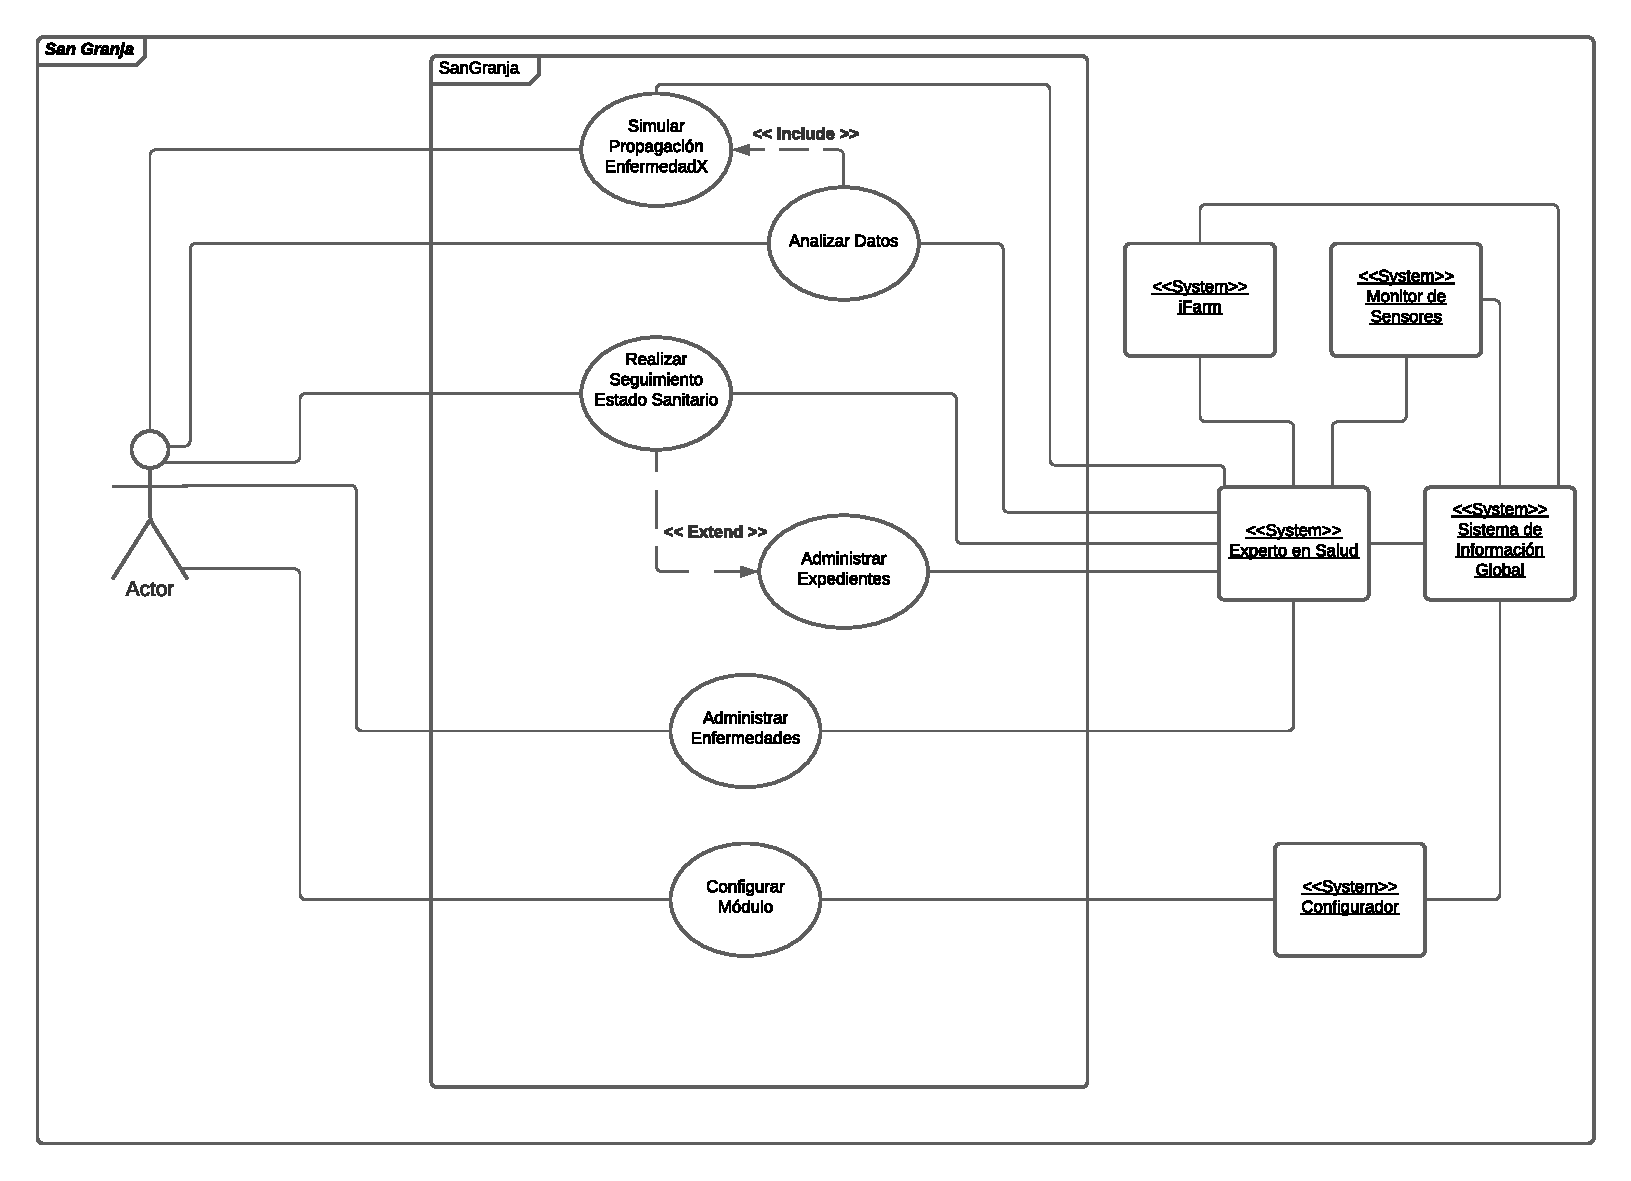
\includegraphics[width=1\linewidth]{graphics/1-MCU.pdf}
	\caption{Evaluación de casos de uso}
\end{figure}


\subsection{Ej 2. (1 punto)}Con la siguiente descripción del  caso de uso  $\ll$SimularPropagaciónEnfermedad\_X $\gg$, escríbalo en un formato completo (se recomienda la variante ‘en dos columnas’) y un estilo esencial (excluyendo los detalles técnicos de nivel bajo). Incluya tanto el flujo en el escenario principal de éxito como 2 extensiones o flujos alternativos que pudieran ser frecuentes:\\
	
	\textbf{Caso de uso:} SimularPropagaciónEnfermedad\_X\\
	\textit{Formato completo (variante ‘a dos columnas’), estilo esencial.}\\
	\textbf{Evolución típica de los acontecimientos}\\
\begin{figure}[H]
	\begin{minipage}[t]{0.48\linewidth}
		\textbf{Acciones del actor}
		\vspace{1em}
		\\
		1 - El usuario ingresa al sistema para realizar \\una simulación sobre una enfermedad definida.
		\vspace{4em}
		\\
		3 - El usuario ejecuta la simulación con los valores por defecto asignados por el sistema para los atributos \textit{número de días}, \textit{corrales} y \textit{vector de contagio} de la simulación.
		\vspace{5em}
		\\
		5- Revisa los resultados y da por terminada la simulación.
		\vspace{2em}
		\\	
		
	\end{minipage}
	\hspace{0.2cm}
	\begin{minipage}[t]{0.08\linewidth}
	\end{minipage}
	\begin{minipage}[t]{0.48\linewidth}
		\textbf{Acciones del sistema}
		\vspace{3em}
		\\
		2 - El sistema muestra los datos de la simulación (corrales, días y  caracterización de la enfermedad con, entre otros datos, su vector de contagio).
		\vspace{6em}
		\\
		4 - El sistema realiza la simulación con los parámetros recibidos, muestra los resultados y pregunta si desea realizar otra simulación.
		\vspace{2em}
	\end{minipage}
\end{figure}
\textbf{Alternativas}
\begin{itemize}
	\item 3a El \textbf{usuario} modifica los valores de los atributos que desea y da comienzo a la simulación, el flujo continúa en \textbf{4}.	
	\item 5b El \textbf{usuario} desea realizar una nueva simulación con valores diferentes, con lo que selecciona dicha opción y pulsa continuar. El flujo sigue desde \textbf{2}.
\end{itemize}

\section{Sección 2.\\Evaluación del Modelado Conceptual}
\subsection{Ej 3. (3 puntos)}

En relación con el  caso de uso anterior,$\ll$SimularPropagaciónEnfermedad\_X $\gg$, construya un Modelo de Dominio y represéntelo en notación UML. Represente los objetos conceptuales,  las  relaciones relevantes entre ellos, su cardinalidad y los atributos candidatos de los objetos.\\

\begin{figure}[H]
	\centering
	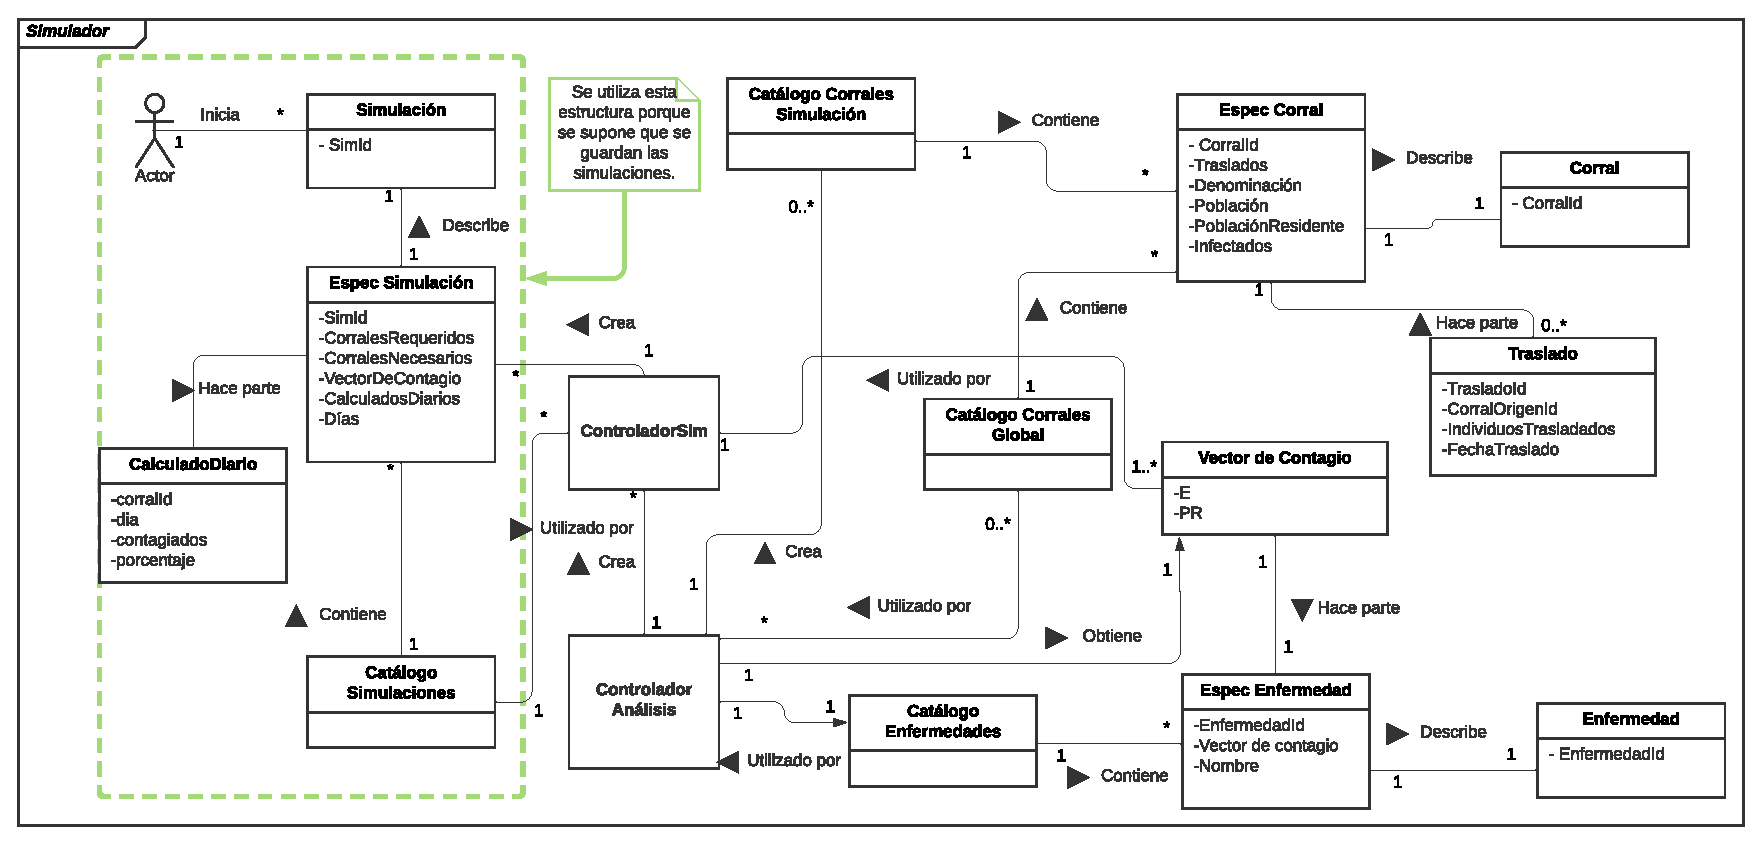
\includegraphics[width=1\linewidth]{graphics/3-MD.pdf}
	\caption{Modelo de Dominio.}
\end{figure}


\section{Sección 3.\\Evaluación de la Asignación de Responsabilidades y Diseño de la Interacción.}
\subsection{Ej 4. (3 puntos)}
Circunscrito al caso de uso  que nos ocupa, $\ll$SimularPropagaciónEnfermedad\_X$\gg$, construya un Diagrama de Interacción en UML. Represente el actor, sus eventos y el paso de mensajes entre cada instancia de las clases software que componen el sistema para este caso de uso.

\begin{figure}[H]
	\centering
	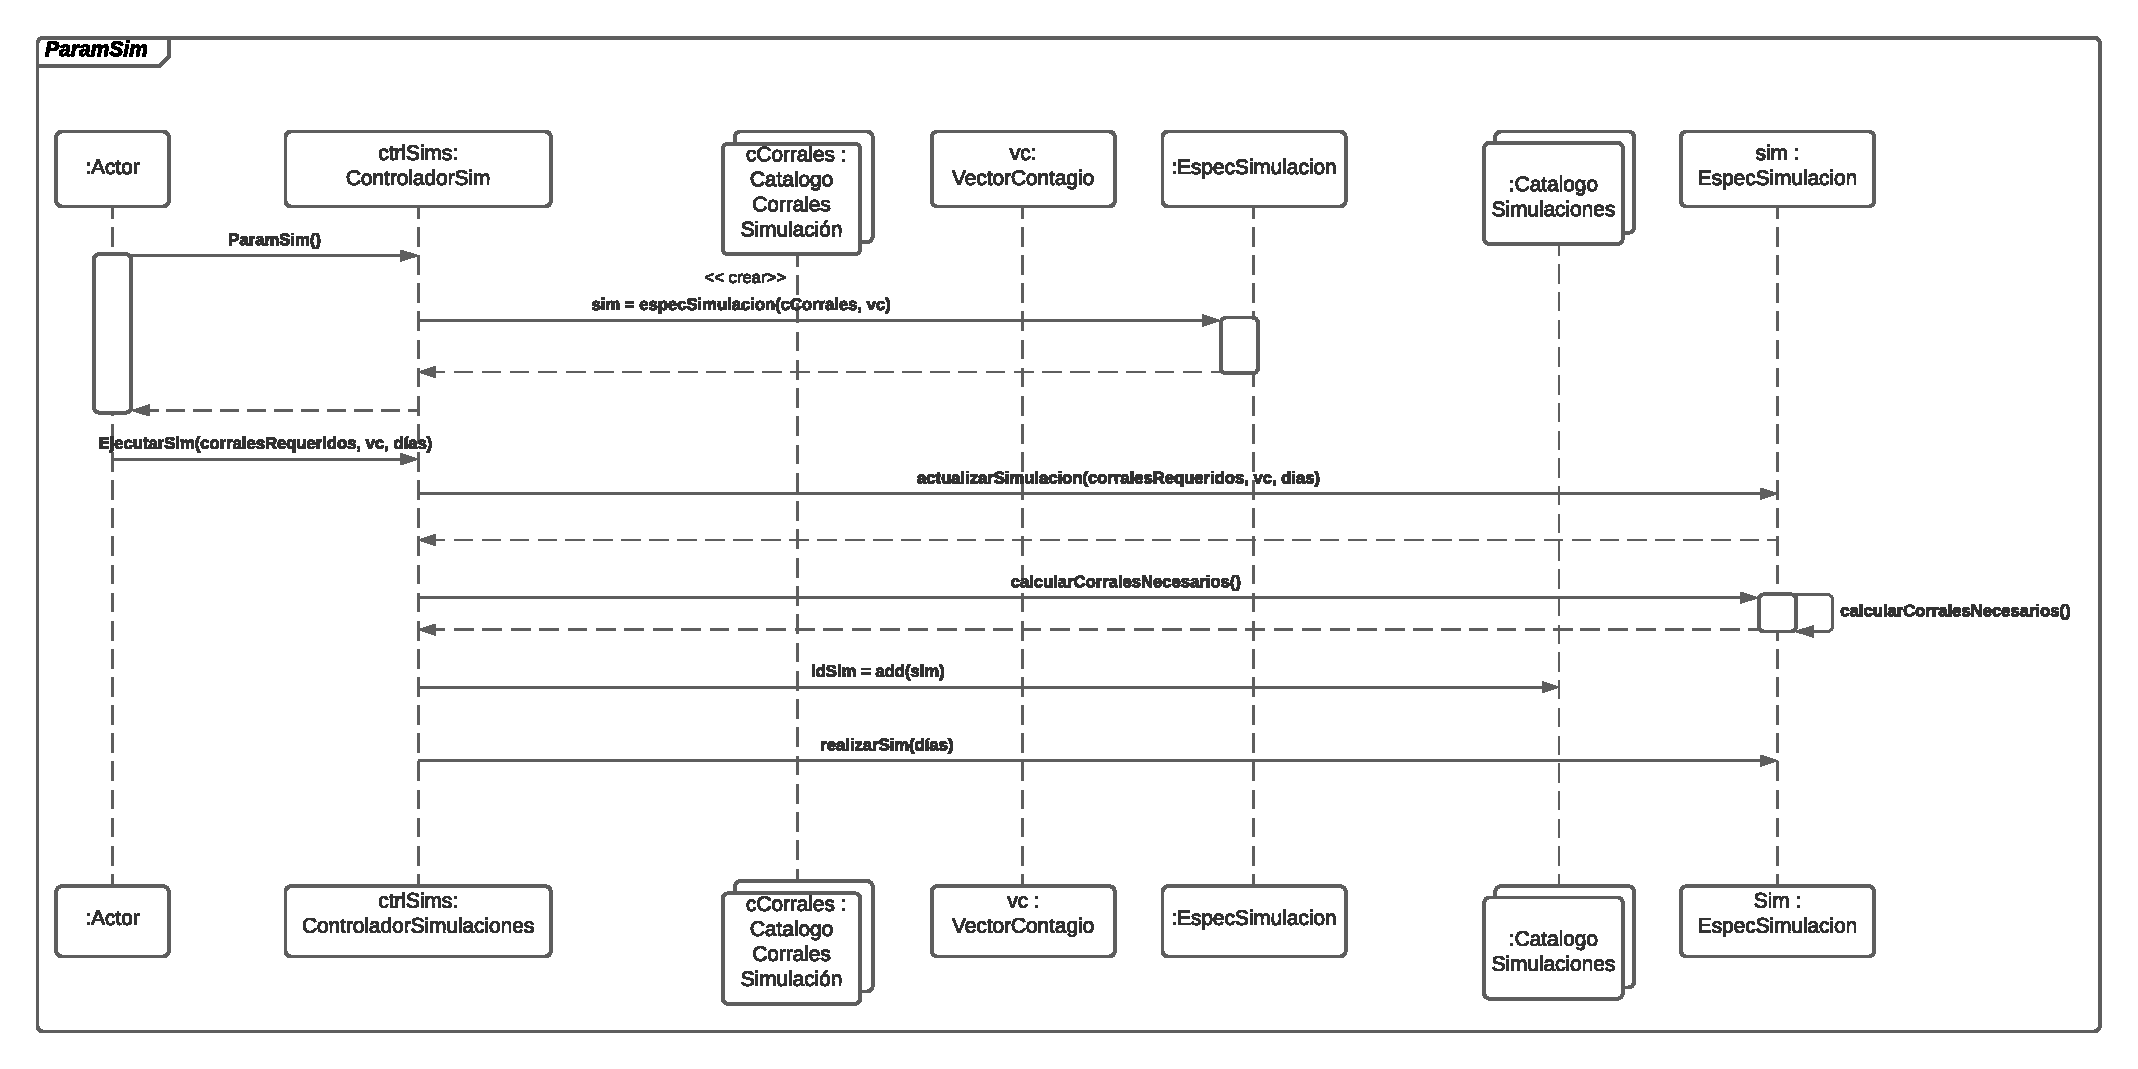
\includegraphics[width=1\linewidth]{graphics/41-DS.pdf}
	\caption{Diagrama de Secuencia ParamSim.}
\end{figure}

\begin{figure}[H]
	\centering
	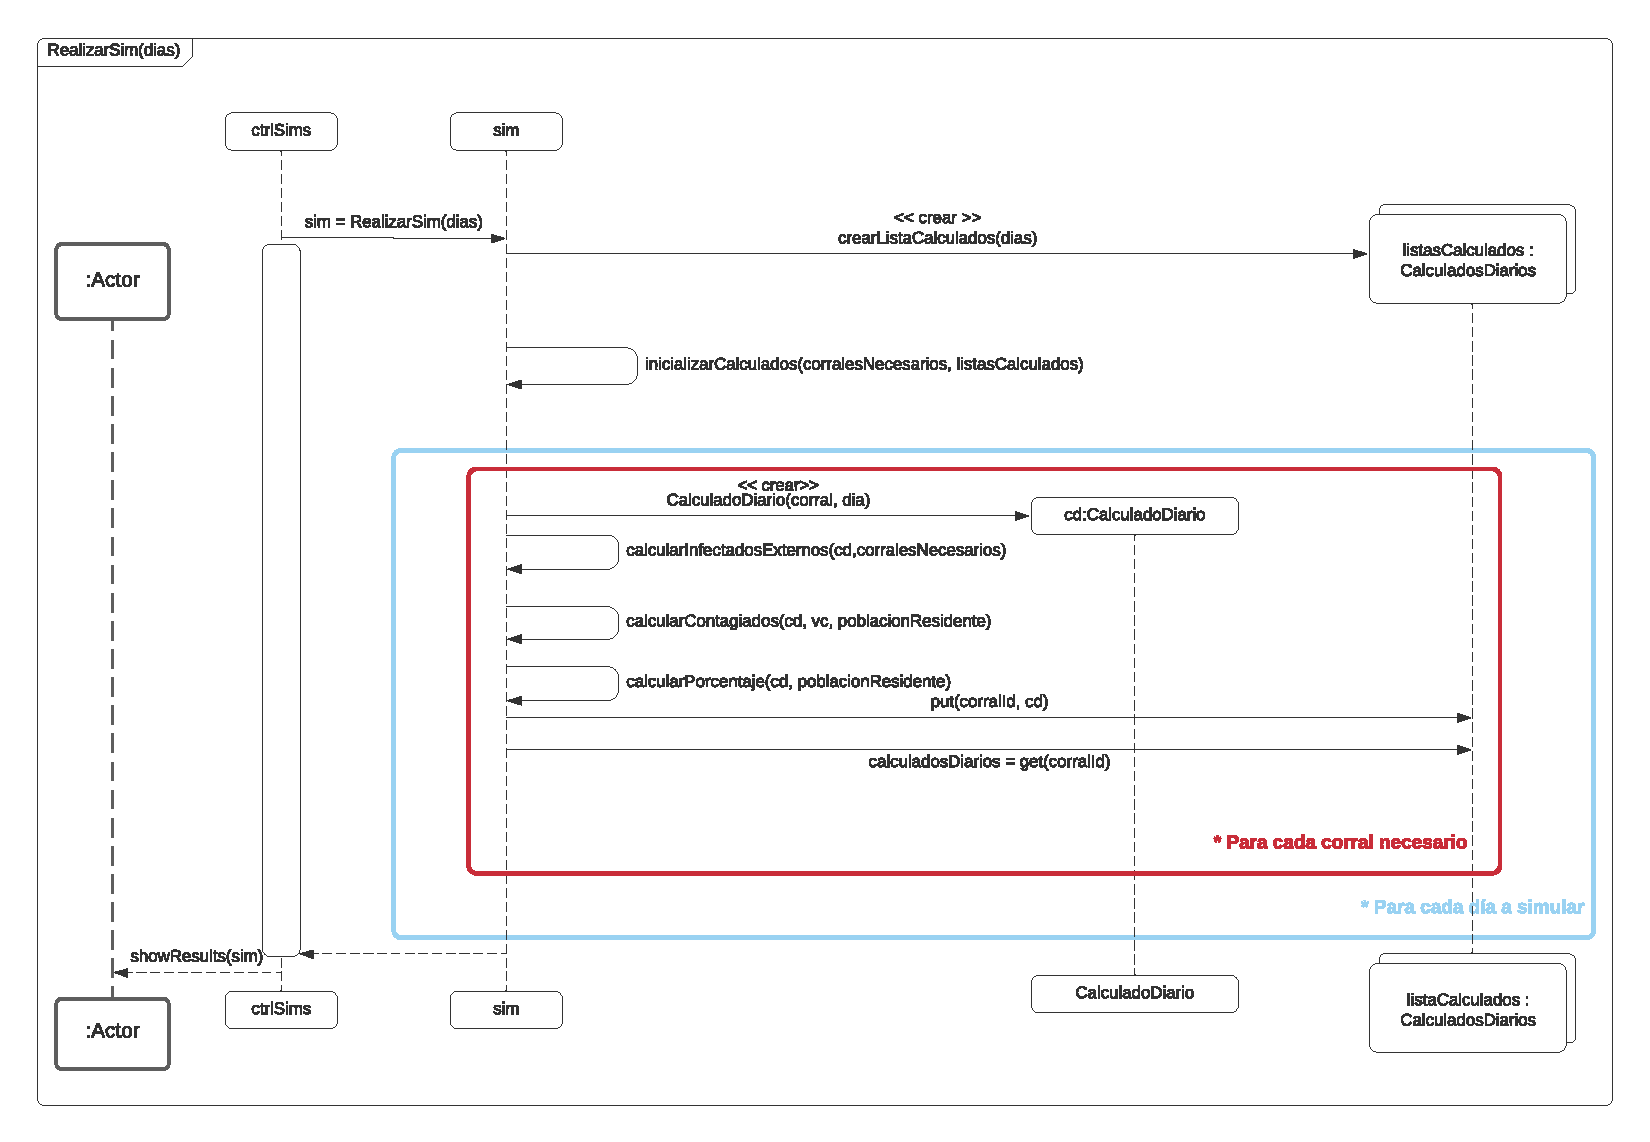
\includegraphics[width=1\linewidth]{graphics/42-DS.pdf}
	\caption{Diagrama de Secuencia RealizarSim.}
\end{figure}

\subsection{Ej 5. (1 punto)}
A partir del Diagrama de Interacción presentado en la pregunta 4, escriba y desarrolle el contrato de la operación ‘\textit{ParamSim}’ que corresponde a la inicialización del caso de uso (la creación e inicialización de las instancias que se requieran en ese momento) y a la asignación de los valores requeridos para realizar los cálculos de la simulación.\vspace{2em}
\\
\textbf{Contrato CO1:} ParamSim
\begin{table}[H]
	\begin{tabular}{ll}
		\textbf{Operación:}	& paramSim()\\		    
	    \\
		\textbf{Referencias cruzadas:} & SimularPropagaciónEnfermedad\_X\\
		\\
		\textbf{Precondiciones:} &Hay una instancia ControladorAnálisis creado.\\	 
		& Hay una instancia ControladorSim creada.\\
		& Hay una instancia del CatálogoCorralesSimulación creado con el cálculo\\ 
		& de la población residente de cada corral realizado.\\
		& Hay una instancia de VectorDeContagio creada, lo que quiere decir que\\ 
		& la enfermedad para la que se realizará la simulación ya ha sido elegida.\\
		& Hay una instancia de CatalogoDeSimulaciones creada.\\
		\\	
		\textbf{Postcondiciones:}
		& Se creó una EspecSimulación, sim con los parámetros por defecto.\\
		& Se actualizó sim, con la información recibida por el usuario.\\		
		& Se rellenó la lista de corrales CorralesNecesarios del objeto sim.\\
		& Se obtuvo el id de la Presa y se asoció a su descripción.\\
		& Se añadió sim  al catálogo de simulaciones.\\	

	\end{tabular}
\end{table}

\section{Sección 4.\\Evaluación del Diagrama de Clases de diseño.}
\subsection{Ej 6. (1 punto)}
Elabore un diagrama de clases para el caso de uso que se está tratando  $\ll$SimularPropagaciónEnfermedad\_X$\gg$  (DCD), centrado en la clase que va a implementar la responsabilidad más característica del caso de uso, la que mejor defina la naturaleza de lo que se hace en él (ControlSim, Calculador, o como lo haya llamado en los diagramas precedentes). Represente los nombres de todos los atributos, asociaciones (con su navegabilidad) y los métodos (excepto ‘setters’ y ‘getters’ irrelevantes), tanto de esa clase como de las que estén directamente involucradas con ella en el funcionamiento del caso de uso.

\begin{figure}[H]
	\centering
	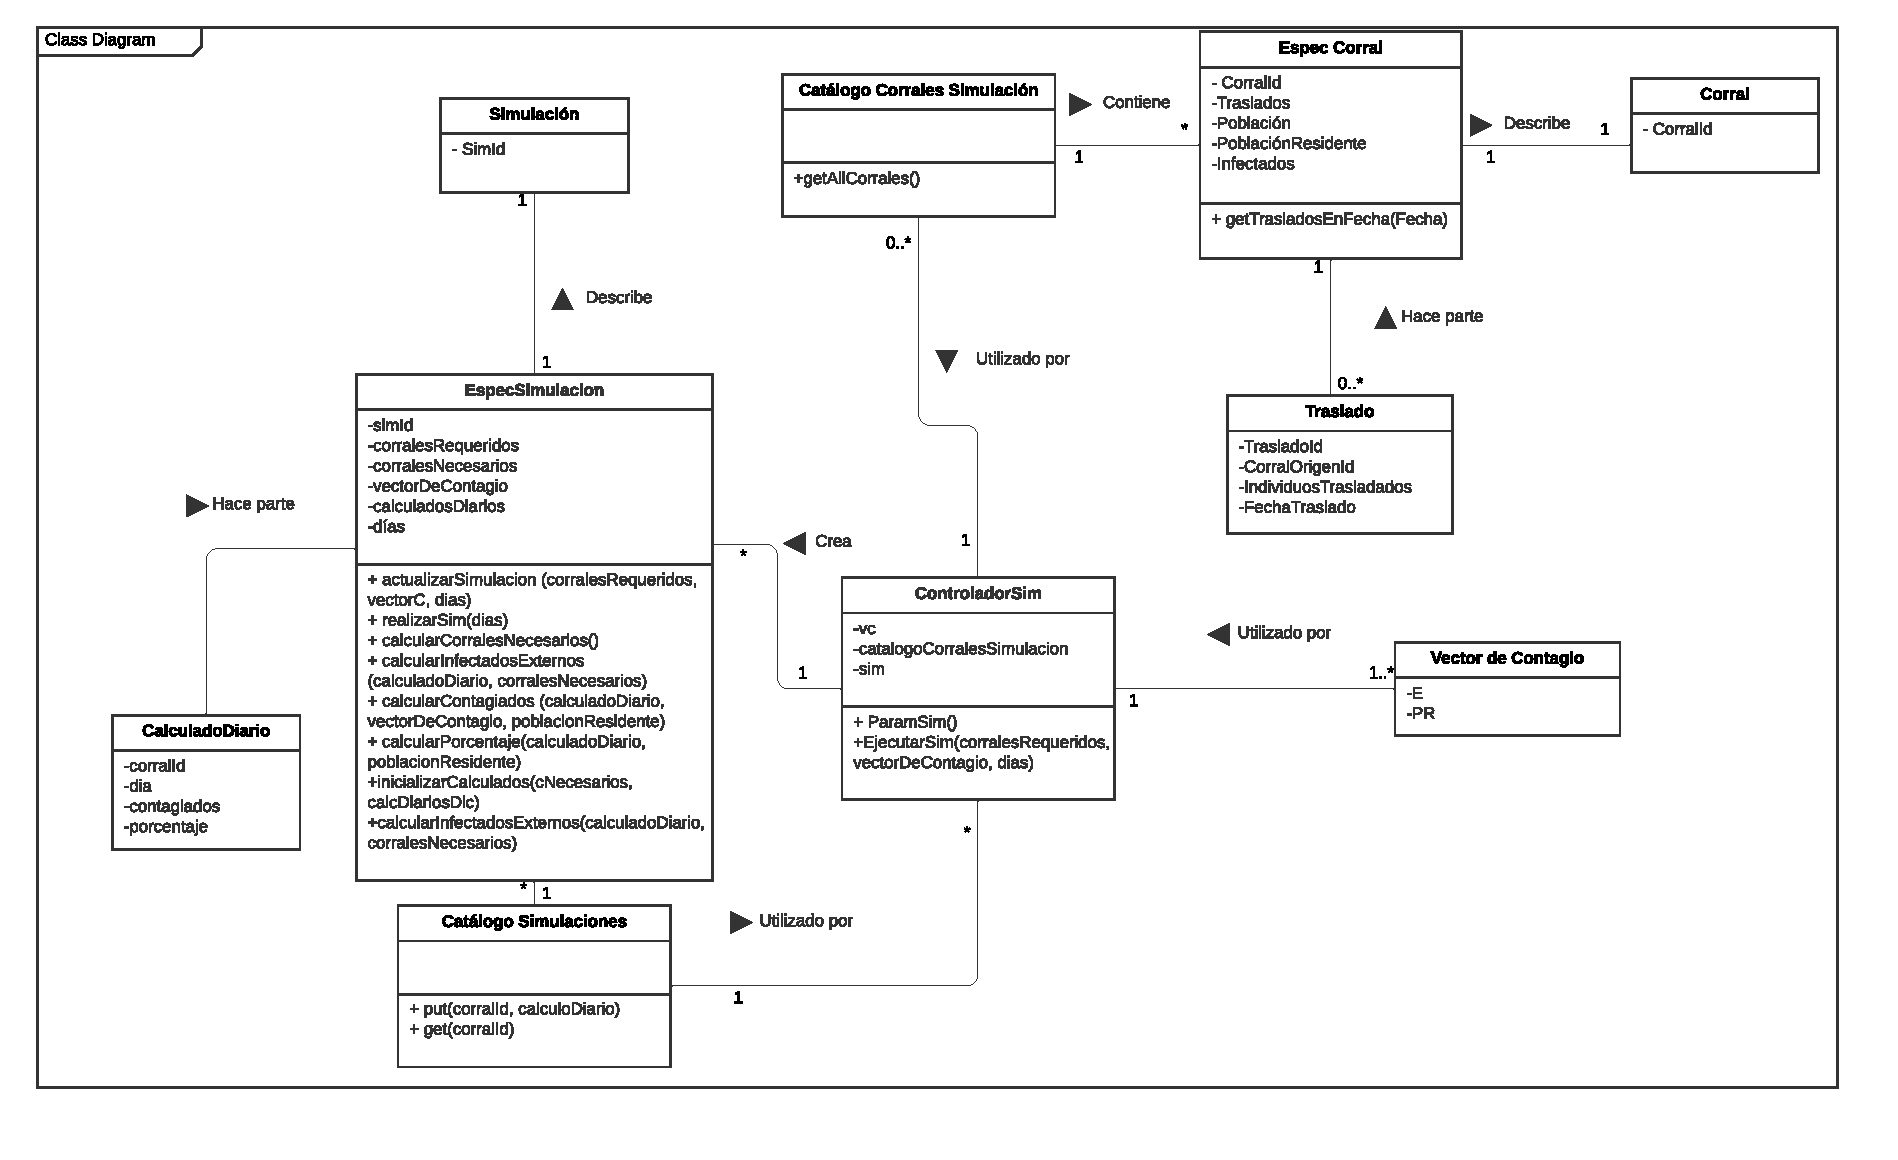
\includegraphics[width=1\linewidth]{graphics/6-DC.pdf}
	\caption{Diagrama de Clases SimularPropagaciónEnfermedad\_X.}
\end{figure}


\section{Sección 5.\\Evaluación de la Transformación del Diseño en Código}
\subsection{Ej 7. (0’5 puntos)}
A partir de los anteriores diagramas de clases y colaboraciones, elabore y defina la clase que haya establecido, en el desarrollo anterior, como responsable de controlar la correcta secuencia de acciones en  el caso de uso $\ll$SimularPropagaciónEnfermedad\_X$\gg$. Incluya las definiciones de todas las variables que la componen (miembros), pero escriba solamente la definición completa del cuerpo para el método principal o los métodos más significativos: $\ll$se omite el método$\gg$. Ignore los pequeños detalles de sintaxis -el objetivo es evaluar la capacidad fundamental para transformar el diseño en código-. Utilice la sintaxis de Java.
\subsubsection{ControladorSim.java}

\begin{lstlisting}
package sanGranja;

import java.util.ArrayList;

public class ControladorSim {

	VectorDeContagio vc;
	CatalogoCorralesSimulacion  catalogoCorralesSimulacion;
	EspecSimulacion sim;	

	public EspecSimulacion ParamSim(){
		this.sim = new EspecSimulacion(catalogoCorralesSimulacion,vc);
		return this.sim;
	}
	
	public void EjecutarSim(ArrayList<Integer> corralesRequeridos,
							VectorDeContagio vc, Integer dias){
		this.sim.actualizarSimulacion(corralesRequeridos, vc, dias);
	}
}
\end{lstlisting}

\subsubsection{EspecSimulacion.java}


\begin{lstlisting}
package sanGranja;

import java.util.ArrayList;
import java.util.Calendar;
import java.util.Date;
import java.util.HashMap;
import java.util.Map;

public class EspecSimulacion {
	
	Long simId;
	ArrayList<Integer> corralesRequeridos;
	HashMap<Integer, EspecCorral> corralesNecesarios;
	VectorDeContagio vectorContagio;
	ArrayList<CalculadoDiario>calculadosDiarios;
	Integer dias;
	
	public EspecSimulacion(CatalogoCorralesSimulacion catalogoCorralesSimulacion,
							VectorDeContagio vc2) {
		catalogoCorralesSimulacion.getAllCorrales().forEach(c->{
			this.corralesNecesarios.put(c.corralId, c);
		});
		this.vectorContagio = vc2;
	}
	
	
	public Long actualizarSimulacion (ArrayList<Integer> corralesRequeridos, 
									VectorDeContagio vectorC, Integer dias)
	{		
		this.corralesRequeridos = corralesRequeridos;
		this.vectorContagio = vectorC;
		this.dias = dias;				
		return this.simId;
	}
		
	public void calcularCorralesNecesarios(){
		ArrayList<EspecCorral> corrales = new ArrayList<EspecCorral>();
		this.corralesRequeridos.forEach( c->{
			corrales.add(this.corralesNecesarios.get(c));
		});
		this.corralesNecesarios.clear();
		corrales.forEach(c->{
			this.corralesNecesarios.put(c.corralId, c);
		});
	}
	
	public void realizarSim(Integer dias){		
		HashMap<Integer, ArrayList<CalculadoDiario>> calculadosDiarios = 
		new HashMap<Integer, ArrayList<CalculadoDiario>>();
		inicializarCalculados(this.corralesNecesarios, calculadosDiarios);
		for (int i = 1; i<=dias; ++i){				
		/*para cada dia, calculo el numero de infectados de cada corral*/
			int dia = i;
			corralesNecesarios.values().forEach( c ->{
				CalculadoDiario cd = new CalculadoDiario(c.corralId, dia);
				Integer contagiadosExternos = 
				calcularInfectadosExternos(cd, this.corralesNecesarios);
				
				Integer contagiados = calcularContagiados(cd, 
				this.vectorContagio, c.poblacionResidente, contagiadosExternos);
				
				cd.contagiados = contagiados;
				Double pct = calcularPorcentaje(cd, contagiados);
				cd.porcentaje = pct;
				ArrayList<CalculadoDiario> listaCalculadosDiario = 
				calculadosDiarios.get(c.corralId);
				
				if (listaCalculadosDiario == null){
					listaCalculadosDiario = new ArrayList<CalculadoDiario>();
				}
				listaCalculadosDiario.add(cd);
				calculadosDiarios.put(c.corralId, listaCalculadosDiario);
				this.calculadosDiarios = calculadosDiarios.get(c.corralId);
			});
		}					
	
	}
	
	private void inicializarCalculados(HashMap<Integer, EspecCorral> cNecesarios,
					 HashMap<Integer, ArrayList<CalculadoDiario>> calcDiariosDic) {
	
		corralesNecesarios.values().forEach( c ->{
			ArrayList<CalculadoDiario> calculadosPorCorral = new ArrayList<CalculadoDiario>();
			CalculadoDiario cd = new CalculadoDiario(c.corralId, c.infectados,
			(double)c.infectados/c.poblacionResidente);			
			calculadosPorCorral.add(cd);
			calcDiariosDic.put(cd.corralId, calculadosPorCorral);
		});	
	}
	
	public Integer calcularInfectadosExternos(CalculadoDiario calculadoDiario,
											  HashMap<Integer, EspecCorral> corralesNecesarios){
		Integer infectados = 0;		
		/*obtengo el dia que estamos calculando */
		Calendar calendar = Calendar.getInstance(); 
		calendar.add(Calendar.DAY_OF_YEAR, calculadoDiario.dia);
		Date fecha = calendar.getTime();
		/*para dicho dia, calculo el numero de infectados de cada corral	*/
		for(Map.Entry<Integer, EspecCorral> entry : corralesNecesarios.entrySet()){
			ArrayList<Traslado> traslados = entry.getValue().getTrasladosEnFecha(fecha);			
			for (int j = 0;j < traslados.size();++j){
				Traslado t = traslados.get(j);
				EspecCorral corral = corralesNecesarios.get(t.corralOrigenId);
				Double porcentaje = (double)corral.infectados/(double)corral.poblacion;
				Double trasladadosInfectados = t.individuosTrasladados.doubleValue() * porcentaje;
				infectados += trasladadosInfectados.intValue();					
			}
			infectados += calculadoDiario.contagiados;
		}
		return infectados;
	}	
	
	public Integer calcularContagiados (CalculadoDiario calculadoDiario, 
		VectorDeContagio vectorDeContagio, Integer poblacionResidente, Integer cExternos){
		//comprobamos que tenemos otros elementos es la lista de calculados diarios de cada corral.
		Integer contagiadosActuales = this.calculadosDiarios.size() == 0 ?
		 this.calculadosDiarios.get(this.calculadosDiarios.size()-1).contagiados: 0;
		 
		Double res = (cExternos *contagiadosActuales * vectorDeContagio.e * vectorDeContagio.pR)
		 * (1 - contagiadosActuales/poblacionResidente);
		 		
		return res.intValue();
	}
	public Double calcularPorcentaje (CalculadoDiario calculadoDiario, Integer poblacionResidente){		
		return (double)calculadoDiario.contagiados / poblacionResidente;
	}	
}
\end{lstlisting}
\pagebreak
\subsubsection{CatalogoCorralesSimulacion.java}
\begin{lstlisting}
package sanGranja;

import java.util.ArrayList;

public class CatalogoCorralesSimulacion {

	ArrayList<EspecCorral> corrales;
	
	public ArrayList<EspecCorral> getAllCorrales()
	{
		return corrales;		
	}
}

\end{lstlisting}
\subsubsection{EspecCorral.java}
\begin{lstlisting}
package sanGranja;

import java.util.ArrayList;
import java.util.Date;

public class EspecCorral {
	Integer corralId;
	ArrayList<Traslado> traslados;
	Integer poblacion;
	Integer poblacionResidente;
	Integer infectados;
	
	/**
	* Devuelve los traslados de un corral para una fecha determinada*/
	public ArrayList<Traslado> getTrasladosEnFecha(Date fecha){
		ArrayList<Traslado> trasladosHoy = new ArrayList<Traslado>(); 
		traslados.forEach(t ->{
		/*Seguramente la comparacion sea diferente, porque solo hay que comparar dia,mes y ano, 
		pero se entiende el concepto.*/
			if (t.fechaTraslado.compareTo(fecha) == 0){
				trasladosHoy.add(t);
			}
		});
		return trasladosHoy;
	}	

	public EspecCorral() {}

}
\end{lstlisting}

\subsubsection{CalculadoDiario.java}
\begin{lstlisting}
package sanGranja;

public class CalculadoDiario {
	Integer corralId;
	Integer dia; 
	Integer contagiados;
	Double porcentaje;
	
	public CalculadoDiario() {
		this.corralId = 0;
		this.dia = 0;
		this.contagiados = 0;
		this.porcentaje = 0.0;
	}
	public CalculadoDiario(Integer cId, Integer dia) {
		this.corralId = cId;
		this.dia = dia;
	}
	public CalculadoDiario(Integer corralId2, Integer infectados,
	double d) {
		this.corralId = corralId2;
		this.dia = 0;
		this.contagiados = infectados;
		this.porcentaje = d;
	}
}
\end{lstlisting}


\subsubsection{VectorDeContagio.java}
\begin{lstlisting}
package sanGranja;

public class VectorDeContagio {
	Double e;
	Double pR;

}

\end{lstlisting}

\subsubsection{Traslado.java}
\begin{lstlisting}
package sanGranja;

import java.util.Date;

public class Traslado {
	Long TrasladoId;
	Integer corralOrigenId;
	Integer individuosTrasladados; /* Cantidad de individuos implicados 
	 en el traslado .*/
	Date fechaTraslado;
}

\end{lstlisting}

\section{Sección 6. Preguntas opcionales BP. Motivación.}
\subsection{Ej 8. (0’5 puntos)}
Indique qué principios GRASP ha utilizado en el ejercicio y qué responsabilidades ha asignado guiándose por ellos.
\paragraph{}
\textit{EspecSimulacion} es un experto ya que contiene toda la información necesaria para saber el resultado del caso de uso en estudio.
\paragraph{}\textit{ControladorAnálisis} es creador ya que se encarga de crear tanto el \textit{ControladorSim} como los objetos que necesita éste para realizar la simulación(\textit{catálogoCorrarlesSimulación} y \textit{vectorDeContagio}). \textit{ControladorSim} también es creador ya que es el encargado de crear y agregar (actualizar) los objetos \textit{EspecSimulacion}.
\paragraph{}Se ha seguido el principio de bajo acoplamiento y alta cohesión al utilizar catálogos de especificaciones de objetos, con esto se logra que no se vean comprometidos los objetos que se comparten con el resto de la aplicación. El hecho de que se genere acoplamiento en la clase \textit{EspecSimulacion} viene dado, principalmente, por la necesidad de que algunos objetos, como el \textit{VectorDeContagio} y los corrales que se necesitan para la realización de la simulación, puedan ser modificados ``localmente'' y que dicha modificación sea inocua para los mismos objetos en el resto de la aplicación.
\paragraph{}Tanto ControladorAnalisis como ControladorSim siguen el patrón Controlador. El primero se encarga de preparar los objetos necesarios para que se pueda llevar a cabo el caso de uso, manejando los eventos del sistema (por ejemplo el manejo del sistema de alarmas que sirve de disparo para la selección de la enfermedad en el caso de uso) y delegando en el controlador de caso de uso cuando ha conseguido los datos necesarios. Por su parte, ControladorSimulacion se encarga de recibir y enviar mensajes al actor y de enviar los mensajes a los obejtos que se encargarán de las operaciones que llevan a cabo el caso de uso.

\subsection{Ej 9. (0’5 puntos)}
Indique qué patrones GoF ha utilizado en el ejercicio y qué mejoras ha obtenido, con su uso, en la elaboración de este desarrollo o en el comportamiento final del código que ha diseñado.
\paragraph{}Al ser un caso de uso reducido, donde la mayor parte de objetos han sido creados antes de entrar al caso de uso, no existen entidades o sistemas externos a los que nos debamos conectar y la resolución es realtivamente sencilla de impolementar, no se han seguido patrones de este tipo y no me ha sido fácil encontrarlos una vez realizada la práctica.


	
	\printindex % Print the index at the very end of the document

\end{document}